\documentclass[a4paper, 10pt]{report}
\usepackage[italian]{babel}
\usepackage[T1]{fontenc}
\usepackage[utf8]{inputenc}
\usepackage{charter}
\usepackage{amsmath}
\usepackage{amsthm}
\usepackage{amsfonts}
\usepackage{graphicx}
\usepackage{wrapfig}
\usepackage{tcolorbox}
\usepackage{fancyhdr}
\usepackage{listings}
\usepackage{longtable}

\usepackage{geometry}
\geometry{a4paper, left=2cm,right=2cm,top=2cm,bottom=2cm}

\pagestyle{fancy}
\lhead{}
\chead{}
\rhead{\bfseries 30 ottobre 2019 }
\lhead{\bfseries Segnali e immagini}

\begin{document}

\begin{longtable}{| p{.15\textwidth} | p{.80\textwidth} |}
\textbf{Cross - correlazione normalizzata 2D} & La crosss - correlazione normalizzata per le immagini è
\begin{align*}
x_1 \otimes x_2(m, n) = \frac{\sum_{u=-k}^{+k} \sum_{v=-k}^{+k} x_1[x_1(u, v)-\overline{x_1}][x_2(u - m, v - n)-\overline{x_2}]}{\sqrt[]{\sum_{u=-k}^{+k} \sum_{v=-k}^{+k} x_1[x_1(u, v)-\overline{x_1}]^2 \sum_{u=-k}^{+k} \sum_{v=-k}^{+k}[x_2(u, v)-\overline{x_2}]^2}}
\end{align*}
\end{longtable}

\subsubsection*{Convoluzione}
\begin{longtable}{| p{.15\textwidth} | p{.80\textwidth} |}
\textbf{Convoluzione} & Dati due segnali continui di variabile reale $f_1, f_2$, l'integrale di convoluzione è
\begin{align*}
f_1 * f_2 = \int^{+\infty}_{-\infty} f_1(\tau) f_2(t - \tau) \, d\tau
\end{align*}

\noindent Praticamente la convoluzione funziona così:
\begin{center}
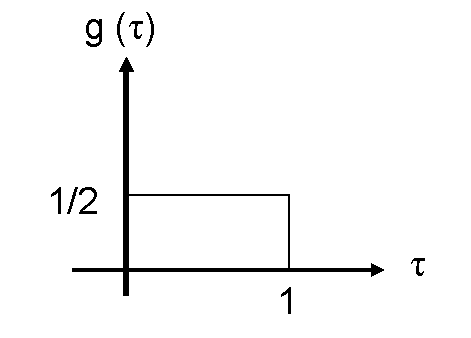
\includegraphics[scale=0.65]{b.pdf}
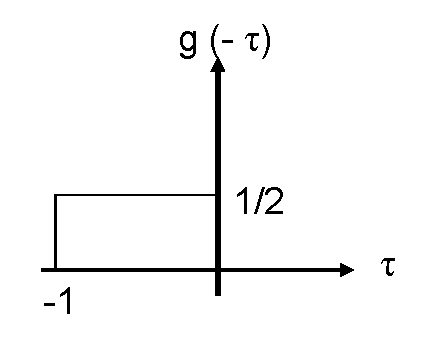
\includegraphics[scale=0.65]{c.pdf}

(Ribalto il grafico $g(\tau)$ rispetto all'origine al fine di ottenere $g(-\tau)$)
\end{center}

\begin{center}
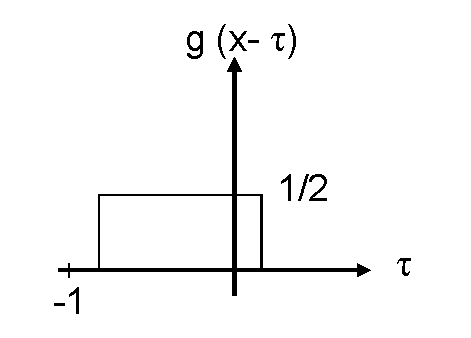
\includegraphics[scale=0.65]{d.pdf}

(Traslo il nuovo grafico di $x$)
\end{center}

\begin{center}
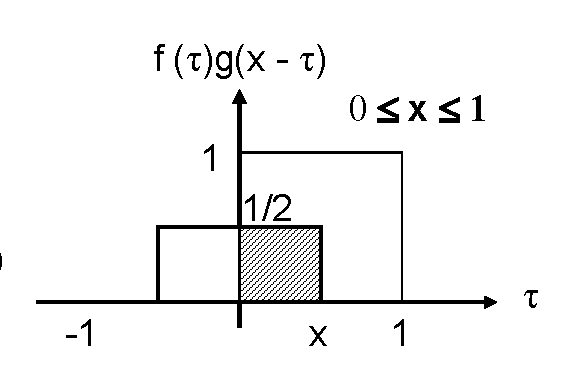
\includegraphics[scale=0.65]{e1.pdf}
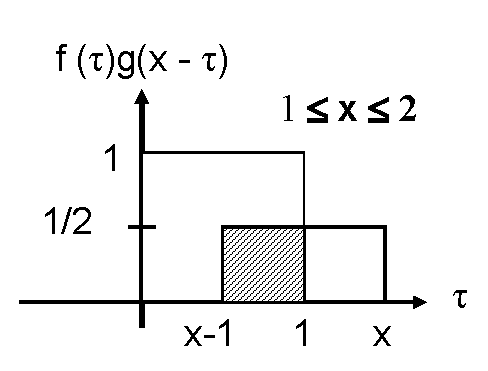
\includegraphics[scale=0.65]{e2.pdf}

(Per ogni valore di $x$, $f(\tau)$ viene moltiplicato per $g(x - \tau)$)
\end{center}
\end{longtable}

\begin{longtable}{| p{.15\textwidth} | p{.80\textwidth} |}
 & 
\begin{center}
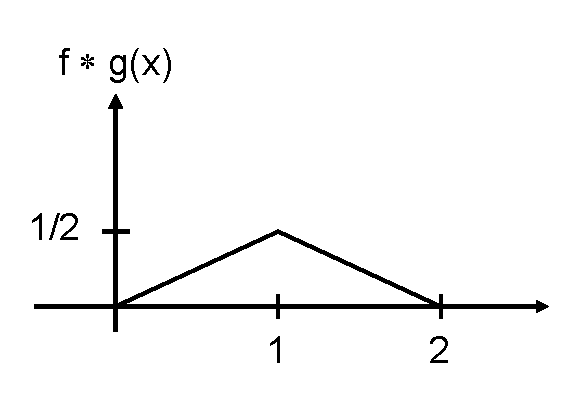
\includegraphics[scale=0.65]{f.pdf}

(Integro il prodotto ottenuto (area grigia))
\end{center}

Se i segnali non sono nè di enerdia nè di di potenza l'integrale diverge.
\\\\
\textbf{Convoluzione discreta} & Nel caso di segnali discreti, la convoluzione diventa
\begin{align*}
x_1*x_2(n) = \sum_{k=-\infty}^{+\infty} x_1(k)x_2(k - n)
\end{align*}
con $k \in Z$ e sotto l'ipotesi di convergenza della serie.

Se $x_1(n)$ e $x_2(n)$ sono limitati di grandezza rispettivamente $M$ e $N$, allora la convoluzione sarà di lunghezza $M+N-1$.
\\\\
\textbf{Convoluzione 2D} & Nel caso di immagini, la convoluzione diventa
\begin{align*}
x_1 * x_2 (n, m) =  \sum_{u=-k}^{+k} \sum_{v=-k}^{+k} x_1(u, v)x_2(n - u, m - v)
\end{align*}

Solitamente il primo segnale viene chiamato filtro (o kernel), mentre il secondo immagine. Solitamente il filtro ha dimensioni minori rispetto al filtro. L'autoconvoluzione non è usata.
\end{longtable}

\underline{Segnali di uso comune}


\end{document}